% https://tex.stackexchange.com/revisions/729888/1
\documentclass[tikz,border=8pt]{standalone}
\usetikzlibrary{positioning}
\usetikzlibrary{chains}
\makeatletter
\tikzset{angle/.code 2 args=\pgfmathsincos{#1}\tikz@lib@place@handle@{#2}{180+#1}{\pgfmathresultx}{\pgfmathresulty}{#1}{1}}
\makeatother

\begin{document}
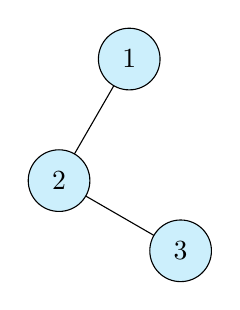
\begin{tikzpicture}[every node/.style={draw, circle, inner sep=5pt, outer sep=0pt, fill=cyan!20}]
    \node (O) {$1$};
    \node (A) [angle={240}{of O}] {$2$} edge (O);
    \node (B) [angle={330}{of A}] {$3$} edge (A);
\end{tikzpicture}

\tikzset{60 below left/.style={angle={240}{#1}}}
\begin{tikzpicture}[
  every node/.style={draw, circle, inner sep=5pt, outer sep=0pt, fill=cyan!20},start chain=going 60 below left,every on chain/.style={join}]
\foreach \v in {1, 2, 3}
  \node[on chain] {\v};
\end{tikzpicture}

\tikz[node distance=2.5cm and 4cm, nodes={draw, circle, minimum size=1.25cm}, on grid]
  \draw ellipse [x radius=4cm, y radius=2.5cm] node (O) {O}
    node foreach \ang in {0, 30, ..., 359}[angle={\ang}{of O}]{\ang};
\end{document}